	\documentclass[12pt]{article}
	\usepackage{color}
	
	% This first part of the file is called the PREAMBLE. It includes
	% customizations and command definitions. The preamble is everything
	% between \documentclass and \begin{document}.
	
	\usepackage[margin=1in]{geometry}  % set the margins to 1in on all sides
	\usepackage{graphicx}              % to include figures
	\usepackage{amsmath}               % great math stuff
	\usepackage{amsfonts}              % for blackboard bold, etc
	\usepackage{amsthm}                % better theorem environments
	\usepackage{changepage}
	\usepackage{lipsum}                     % Dummytext
	\usepackage{xargs}  
	\usepackage{amssymb}                    % Use more than one optional parameter in a new commands
	\usepackage[pdftex,dvipsnames]{xcolor}  % Coloured text etc.
	% 
	\usepackage[colorinlistoftodos,prependcaption,textsize=tiny]{todonotes}
	\newcommandx{\unsure}[2][1=]{\todo[linecolor=red,backgroundcolor=red!25,bordercolor=red,#1]{#2}}
	\newcommandx{\change}[2][1=]{\todo[linecolor=blue,backgroundcolor=blue!25,bordercolor=blue,#1]{#2}}
	\newcommandx{\info}[2][1=]{\todo[linecolor=OliveGreen,backgroundcolor=OliveGreen!25,bordercolor=OliveGreen,#1]{#2}}
	\newcommandx{\improvement}[2][1=]{\todo[linecolor=Plum,backgroundcolor=Plum!25,bordercolor=Plum,#1]{#2}}
	\newcommandx{\thiswillnotshow}[2][1=]{\todo[disable,#1]{#2}}
	
	% various theorems, numbered by section
	
	\newtheorem{thm}{Theorem}[section]
	\newtheorem{lem}[thm]{Lemma}
	\newtheorem{prop}[thm]{Proposition}
	\newtheorem{cor}[thm]{Corollary}
	\newtheorem{conj}[thm]{Conjecture}
	
	\DeclareMathOperator{\id}{id}
	
	\newcommand{\bd}[1]{\mathbf{#1}}  % for bolding symbols
	\newcommand{\RR}{\mathbb{R}}      % for Real numbers
	\newcommand{\ZZ}{\mathbb{Z}}      % for Integers
	\newcommand{\col}[1]{\left[\begin{matrix} #1 \end{matrix} \right]}
	\newcommand{\comb}[2]{\binom{#1^2 + #2^2}{#1+#2}}
	\usepackage{graphicx}
	\usepackage{csquotes}
	\usepackage{lipsum}
	\newcommand\tab[1][1cm]{\hspace*{#1}}
	
	\begin{document}
		
		
		\nocite{*}
		
		\title{Colloquium Attendance \#2: Knotting and linking in spatial graph embeddings \\ By Kenji Kozai}
		
		
		\author{Ziv Epstein \\ 
			\texttt{ziv.epstein@pomona.edu}}
		
		\maketitle
		
		%Attend at least two colloquiums—Wednesdays at 4:15 at CMC, cookies at 3:45—or research seminars this semester and write a paragraph about each talk. Your paragraph can be about the topic of the colloquium or the strengths and weaknesses of the presentation style. We urge you to go to colloquiums early in the semester, since you may decide that you want to go to more than the required two! Ideally, you will submit your paragraph no later than two days after the talk. However, we will accept them up to ten days after the talk.
		\textbf{Topic}: This talk discusses the notion of embedding an abstract graph in $\mathbb{R}^3$, with vertices as points in $\mathbb{R}^3$ and edges as arcs.
		
		The talk starts with a theorem by Conway and Gordon that states that every embedding of $K_6$ has a disjoint pair of 3-cycles that are linked.
		
		Then, it introduces a\textbf{ linking number}, a measure of complexity for a loop. The measure is independent of ambient isotopy and projection and is an link invariant. 
		Then it contends that every embedding of a $K_7$ has a non-trivial knot. It then moves onto the existence of 3d knots in biology. There is an entire characterization of knots, but only some occur in nature. Is there an underlying generator?
		Nick Pippinger proved in '89 that the probability that a closed lattice walk of length $n$ is unknotted is approximately $C^n$ for some $0<C<1$ for large $n$. Which is to say it gets knotted exponentially fast. The Flapan-Kozai introduces the idea of a writhe, which is the coolest name for a mathematical concept I have heard.
		
		\textbf{Strengths}: Very clear, fluid and engaging lecturer. Gave a very good overview of the field and the main results, with added discourse on why these results are important and foundational. Very nice. 
		
		\textbf{Weaknesses:} The proofs Kozai walked through are not visual, despite using a highly visual proof technique. He just talked them out. This highly visual theorem could benefit from visual aids to hammer in the intuition.
\begin{figure}
	\centering
		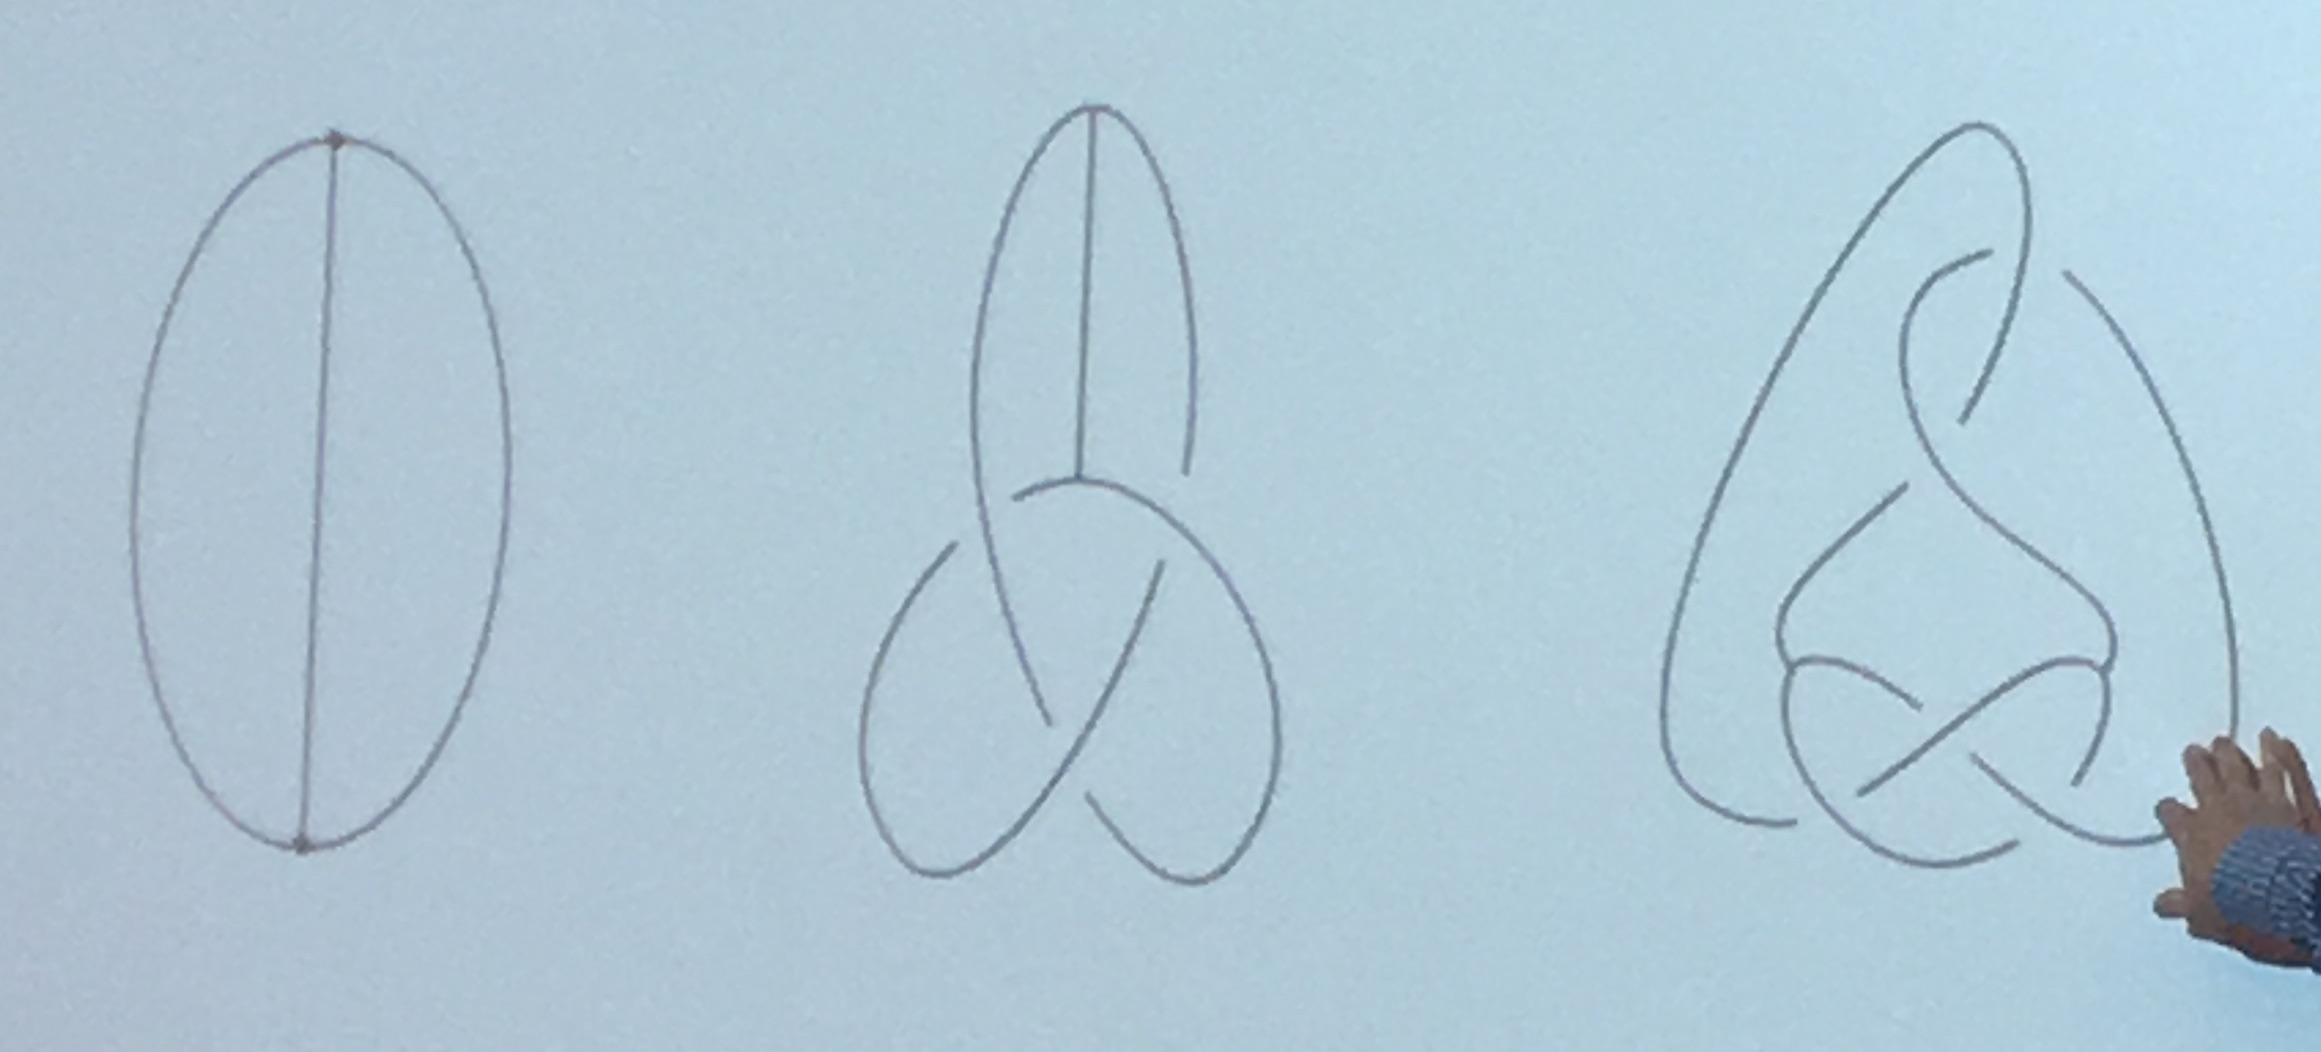
\includegraphics[width=10cm]{knots.JPG}
\end{figure}		
I asked a question about embedding large networks in $\mathbb{R}^3$ and his response was not very helpful.
	
		
	\end{document}